\chapter{预备知识}\label{chap:pre-knowleage}

本章节将以规约 \textit{Client\_Server} (图\ref{fig:client_server})为例,
介绍 \TLA 规约的基本结构,以及在寻找归纳不变式过程中的其他预备知识。
\begin{figure}
    \centering
    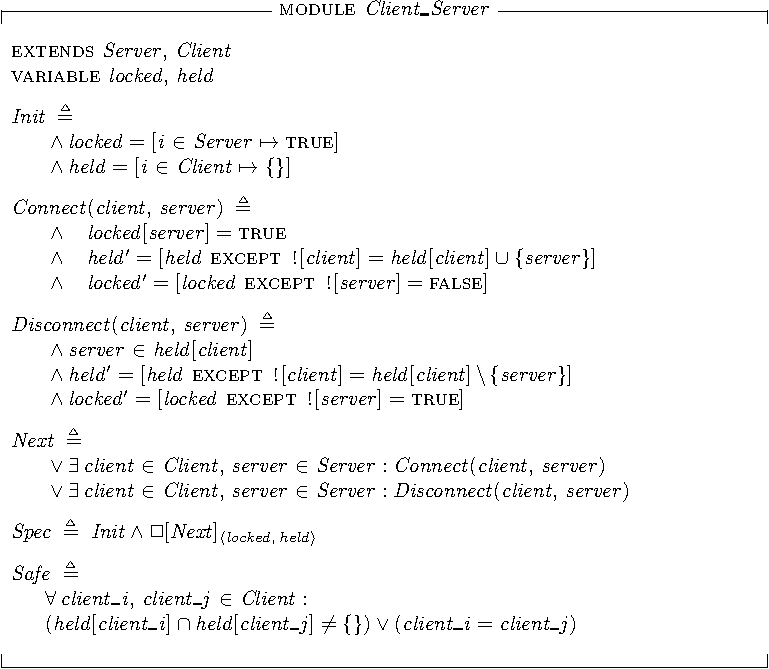
\includegraphics[width=0.8\textwidth]{figures/Client_Server.pdf}
    \caption{Client\_Server 规约}
    \label{fig:client_server}
\end{figure}

\section{\texorpdfstring{TLA\textsuperscript{+}}{TLA+}}
\href{https://lamport.azurewebsites.net/tla/tla.html}{\TLA} \cite{TLA}是由计算机科学家 Leslie Lamport 主导开发的,
用于对计算机程序和系统建模,尤其是对并行系统和分布式系统建模的高级语言。
它是基于使用简单的数学语言来精确描述系统行为的理念开发的。
因此,\TLA 的表达方式和一般的编程语言有很大的不同,反而和数学语言更为接近。
\TLA 并不是一种编程语言,而是一种规约语言,它不关注协议或者系统的具体实现,从而能更高层次看到程序整体的设计。
因此,\TLA 及其工具对于消除代码中很难发现和纠错成本高昂的错误非常有用。

需要注意到的是,\TLA 并不是为了寻找归纳不变式而设计的,而是为了对系统进行建模,是为了让规约开发人员能更好地表达一个协议。
它的语法更加丰富,以更加直观的方式表达一个协议。

开发者使用 \TLA 或者其他工具来对分布式协议进行建模的代码,我们将其称之为规约(specification,简称spec)。
图 \ref{fig:client_server} 展示了一个简单的 \TLA 规约,其中包含了一个简单的客户端和服务器的通信协议。
其中两个重要的谓词是 $Init$ 和 $Next$。
$Init$ 表示系统的初始状态,描述系统最开始时的状态;
而$Next$ 则是表示系统的状态是如何转移,也就是系统的状态在每个时间片后会发生怎样的变化。
在这个规约中,其他的谓词还有$Connect, Disconnect$ 等,定义这些谓词,就像在一般的编程语言中定义函数一样,方便阅读和重复使用。
一些规约中还有谓词 $TypeOK$,用于约束变量的类型。
另一种在自动归纳不变式生成研究中常常使用的工具,IVy,也有相似的语法和结构。
可以看到的是,\TLA 更关注系统的状态和系统状态是发生怎样的转移,对于系统状态转移的具体实现,\TLA 并不关心。
这样的描述方式和状态机非常相似。

谓词$Safe$ 是安全属性(safety property),一个正确定义的分布式协议规约,应当在每个可达的状态下都满足安全属性。
这个变量在自动化生成归纳不变式的研究中非常关键。

TLC 是 \TLA 集成的模型检测工具。
除了 TLC 以外,\TLA toolbox\cite{tla+toolbox} 还集成有PlusCal\cite{PlusCal}和TLAPS用于命题证明工具,sany用于语法检查工具,
tex 用于将\TLA 美化打印的工具等,这些工具与本文所讨论的问题相关性不高,不展开讨论。

本文所述工具接受\TLA 的规约。

\section{归纳不变式和归纳反例}
验证分布式协议的正确性,就是验证协议定义的安全属性(safety property)是否在每个可达的状态下都成立。
在 \textit{Client\_Server} 规约中,我们可以看到 $Safe$ 是一个安全属性,
它表达的是,在任何状态下,如果两个客户端同时连接有同一个服务器,那么这两个客户端是同一个客户端。
换言之,两个不同的客户端不能连接到同一个服务器。

对于简单的系统,即变量和状态不多的系统,我们可以通过遍历每一个可能的状态来验证。
但是对于稍微复杂一些的系统,尤其是越来越多的分布式系统,规模越来越大,状态也越来越复杂。
通过简单的遍历的方式来验证系统的正确性,是不现实的。
寻找一个能够蕴含安全属性的不变式,并且能够在所有可能的状态转移后保持其自身的正确性,这个不变式被称为归纳不变式。
以数学的语言表示为:
\begin{align}
    &Init \Rightarrow Ind \label{con:init}\\
    &Ind \land Next \Rightarrow Ind' \label{con:inductive}\\
    &Ind \Rightarrow Safe \label{con:safety}
\end{align}
其中$Init$ 表示初始状态,$Next$ 表示状态转移,$Safe$ 是安全属性,$Ind$ 表达的是归纳不变式,
而$Ind'$表达谓词$Ind$经过状态转移后的变量的状态。
定理\ref{con:init}表明归纳不变式在初始状态下成立;
定理\ref{con:inductive}表明归纳不变式在状态转移后依然成立,具有归纳性质。
比如说,如果$Ind$在状态$s$下成立,那么在$s$的后继状态下,$Ind$依然成立;
定理\ref{con:safety}表明归纳不变式蕴含安全属性,因此,如果某个运行时可达状态满足$Ind$, 那么也必然满足$Safe$。
这是我们寻找一个这样的归纳不变式的目的,通过归纳不变式的正确性验证安全属性的正确性。
这是归纳不变式所必须满足的三个条件。

\begin{align}
    &\left.A_{1} \triangleq \forall s \in  { Server }: \forall c \in  { Client }:  { locked }[s] \Rightarrow(s \notin { held }[c])\right) \\
    &{ Ind } \triangleq  { Safe } \wedge A_{1} \label{con:candidate_ind}
\end{align}

对于\textit{Client\_Server} 规约,表达式\ref{con:candidate_ind}是一个可能的归纳不变式。
可以看到的是,$Ind$是由$Safe$和$A_{1}$两个谓词逻辑表达式合取组成而来。
事实上,大部分规约的归纳不变式都可以表达为$Ind \triangleq Safe \wedge A_1 \wedge A_2 \wedge... \wedge A_n$的形式。
其中合取子式$A_k$是约束状态的谓词,我们将之称为引理不变式(Lemma Invariant)。
因为归纳不变式$Ind$是由这些引理不变式$A_k$组合而成的,也就是说,归纳不变式强于每一个引理不变式。
因此,引理不变式需要满足不变性,也就是在系统运行的每个状态下都成立,才能成为一个合适的引理不变式。
但是,引理不变式本身不需要满足归纳性,只需要他们和安全属性的合取结果能够满足归纳性。

对于一个谓词表达式$P$,如果一个状态$s$满足$s \models P$,但是$s$的后继状态$s_{n} \models \neg P$,
那便可以称$s$ 为 $P$的归纳反例(counterexample),揭示了$P$不是归纳不变式。
一个归纳反例往往包括两个状态,前一个状态满足谓词$P$,而后一个状态不满足谓词$P$。

\begin{figure}
    \centering
    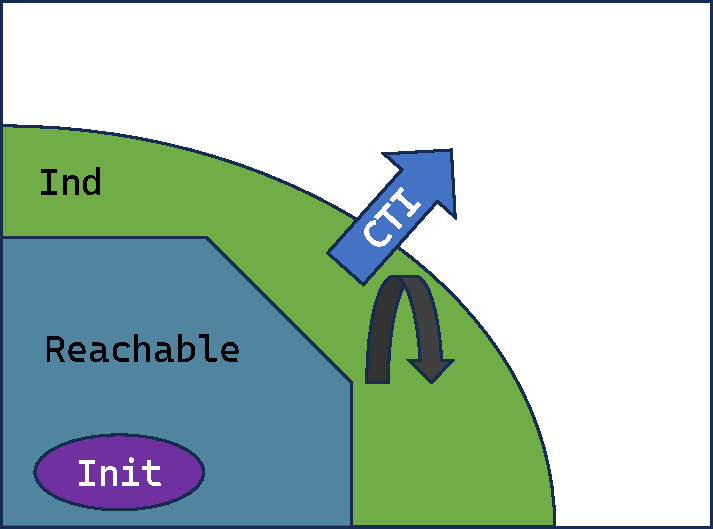
\includegraphics[width=0.7\textwidth]{figures/ind-cti.pdf}
    \caption{归纳不变式和归纳反例}
    \label{fig:ind-cti}
\end{figure}
图\ref{fig:ind-cti}形象地介绍了归纳不变式和归纳反例。
寻找归纳不变式的过程,也可以理解为通过添加新的引理不变式,来排除归纳反例的过程。
但是,尤其是对于越复杂的系统而言,寻找归纳不变式并不是一个简单的任务。
实现归纳不变式的自动生成是形式化验证领域一个重要的研究目标,这也是本文研究的内容。

\section{TLC 和 Apalache}
TLC和Apalache是两个常见的面向\TLA 规约的模型检查工具(model checker)。
本文通过TLC和Apalache来验证生成的候选不变式的性质。
主要是借助TLC或Apalache获取归纳反例,以及验证生成模块生成的谓词表达式是否是有限实例上的不变式。

\subsection{TLC}
TLC既是对\TLA 规约的模型检查工具,也是一个面向规约的模拟器。
它是一个显式状态模型检查器,依照用户给出的规约和设置,搜索所有满足约束的状态和状态转移,
并在这个过程中检查安全属性和其他用户定义的谓词逻辑时时是否成立。
如果遇到错误,TLC会将错误的状态和状态转移过程输出,以便用户进行分析。

TLC可以通过使用超过32个计算机线程以获得近乎线性的加速。
它可以通过在分布式部署的计算机网络上运行来进一步加速模型检查,并提供在云系统上的轻松部署。

\subsection{Apalache}
Apalache\cite{apalache1, apalache2} 和 TLC 不同的是,Apalache 并不是通过遍历所有可能的状态来检验安全属性是否成立,而是通过 SMT solver 来检验。
它是将\TLA 规约转换为 SMT 问题,然后使用 SMT solver (如Z3\cite{z3})求解来检验安全属性是否成立。
Apalaches 是一种符号检查器,它和 SMT solver 一样基于逻辑推理和公式求解实现的。
Apalache 对\TLA 源文件的语法中引入了一些限制,
尽管没有完全支持\TLA 的所有语法,但是这方便使用 SMT 求解器进行求解。

\TLA 是一个“弱类型”的编程语言,它对变量没有严格的类型注明。
但是,Apalache 需要了解\TLA 规约中变量的类型才能工作。
尽管 Apalache 有一套自己的类型推断系统,但是,它并不能完全解决所有的类型推断问题。
这使得用户,对于某些协议,需要以注释的形式来提供变量的类型,才能交给Apalache进行处理。

% 补充关于 返回结果和CTI的内容?

\section{强化学习}
强化学习(Reinforcement learning, RL)\cite{rl}是机器学习的一个领域,强调如何基于外部环境做出决策,以获得最大化的预期累积奖励。
是区别于监督学习和非监督学习的另外一种基本的机器学习方法。
强化学习的关注点在于寻找对未知领域的探索和对已有知识的利用之间的平衡。
它的目标是通过奖惩来控制智能体完成任务,以获得最大化的预期累积奖励,但程序无需明确告诉智能体如何完成任务。

在机器学习问题中,环境通常被抽象为马尔可夫决策过程(Markov decision processes,MDP)\cite{markov},
因为很多强化学习算法在这种假设下才能使用动态规划的方法。
传统的动态规划方法和强化学习算法的主要区别是,后者不需要关于MDP的知识,而且针对无法找到确切方法的大规模MDP。

\begin{figure}[h]
    \centering
    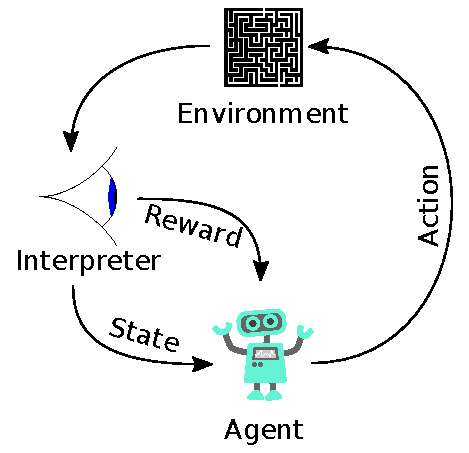
\includegraphics[width=0.6\textwidth]{figures/Reinforcement_learning_diagram.pdf}
    \caption{强化学习框架}
    \label{fig:rl}
\end{figure}
图 \ref{fig:rl} 展示了强化学习的框架。
强化学习中,主要是智能体(agent)和环境(environment)之间的交互。
环境是智能体所处的环境,它会根据智能体的动作,给予智能体奖励或者惩罚,并作出状态转移。
智能体根据奖励和环境状态的变化来调整自己的策略。
智能体,可以感知环境的状态(State),并根据反馈的奖励(Reward)学习选择一个合适的动作(Action),来最大化长期总收益。
智能体会根据环境的反馈,调整自己的策略,以获得最大化的预期累积奖励。
实现强化学习的策略算法有很多,其中最著名的有 Deep Q Network(DQN)\cite{dqn},Q-learning\cite{q-learning}等。

在本文的项目中,我们使用强化学习的方法来加速归纳不变式的生成。
我们使智能体理解\TLA 原文件的内容,让智能体合理选择生成归纳不变式的种子(seed),
并将每一次智能体选择的种子所生成的不变式的检验结果反馈给智能体,包括反例的数量,内容和生成时间等。
智能体根据这些反馈信息,调整自己的策略,以便更快地找到一个满足安全属性的归纳不变式。

